\begin{center}
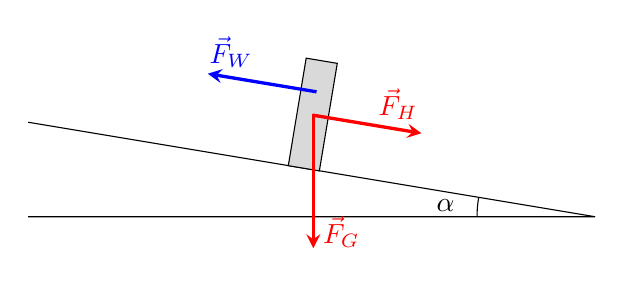
\begin{tikzpicture}[>=stealth]
 \draw (0,1.2) -- (7.2,0) -- (0,0);
 \draw (5.7,0) arc (180:170.5:1.5);
 \node at (5.3,0.14) {$\alpha$};
 \begin{scope}[rotate around={-9.46:(3.5,0.616)}]
  \draw[fill=gray!30] (3.3,0.616) rectangle (3.7,2.0);
  \draw[->, very thick, red] (3.5,1.3) -- (4.9,1.3);
  \node[red, above] at (4.6,1.3) {$\vec F_\text{H}$};
  \draw[->, very thick, blue] (3.5,1.6) -- (2.1,1.6);
  \node[blue, above] at (2.4,1.6) {$\vec F_\text{W}$};
 \end{scope}
 \draw[->, very thick, red] (3.62,1.3) -- (3.62,-0.4);
 \node[red, right] at (3.62,-0.2) {$\vec F_\text{G}$};
\end{tikzpicture}
\end{center}

Ein Gefälle von $p = \pInO$ bedeutet $\tan\alpha = p$, also
\begin{align}
 \alpha &= \alInF = \alIn
\end{align}
Die Skaterin wird schneller, bis die Luftwiderstandskraft so gross ist wie die Hangabtriebskraft $F_\text{H} = m\,g\sin\alpha$ (die Normalkraft und die Komponente der Gewichtskraft senkrecht zur Strasse heben sich auf):
\begin{align}
 \frac{1}{2}\,c_w\,\rho\,A\,v^2 &= m\,g\sin\alpha
\end{align}
Mit $c_w = \cwMO$ für eine aufrechte Person (FoTaBe S.~189) und $\rho = \rhLO$ (FoTaBe S.~187) ist die Endgeschwindigkeit
\begin{align}
 v &= \vInF \\
   &= \sqrt{\frac{2\cdot\mIn\cdot\gE\cdot\sin\left(\alIn\right)}{\cwM\cdot\rhL\cdot\AIn}} \\
   &= \vIn \approx \result{\vInP{0}{2}} = \result{\vInkP{0}{2}}
\end{align}
